\chapter{Oasis Local Db}
\label{ch:Db}
In this chapter we describe the local database, called Oasis Local Db. Oasis Local Db is used for saving the data, which is used by the GIRAF applications. First the structure of Oasis Local Db is described in section \vref{sec:dbStruc}. After that the implementation of Oasis Local Db on the android system is described in section \vref{sec:dbImp}.

\section{Structure}
\label{sec:dbStruc}
The structure of Oasis Local Db is developed in cooperation with the savannah server group. The reason for that is to alleviate the complexities that could occur during a synchronization of the tablet and the savannah server. 

The central point of the database schema is the AuthUsers table.
This table contains all the user id's and their certificates.
A user in the database can be either a profile or a department and therefore a role is stored as well to differetiate the two.

The database schema for the profiles and departments are a simple model representing a kindergarden like Birken or Egebakken.
This means that a profile can either be a child, a pedagouge, or a parent.
The database supports the possibility to associate profiles to each other in order to allow a child to guardian relation.
The profiles can be attached to one or more departments, and a department can be related to one or more sub departments.

An important part of the system for the guardians is the ability to access different kinds of media on the tablets.
Therefore media can be stored in the database along with information about who has access to them.
A media can be owned by either a profile or a department, and the owner has the ability to decide who should have access to the media.
The database schema also allows the user to adds tags to media, these tags can be used to identify the media.

Another important part of the system is the ability to control appplications.
From the users viewpoint it consists of deciding which applications should be accessible and from the developers viewpoint it is a way of saving application settings for a profile.

The database schema can be seen in figure \autoref{fig:localDatabaseDesign}.


There are a few differences between our database schema and the savannah database schema. The reason for that is that there only is SQLite, which is embedded into the Android system. SQLite is an open source database. It supports three kinds of data types; TEXT, which is similar to String type in Java, INTEGER, which is similar to long type in java, and REAL, which is similar to double type in java. SQLite does not validate if the types written to the columns actually are of the defined type. This means that it for instance is possible to write an integer into a TEXT column. On the positive site SQLite only requires a little portion of memory at runtime (~250 KByte). Kilde:

When making a SQLite Database on an Android device it is only needed to define the SQL statements for creating and updating the database. After that the Android system will manage it. An example of how we implemented a table in the database can be seen in section \vref{dbImp}.

\begin{figure}[htbp]
	\centering
		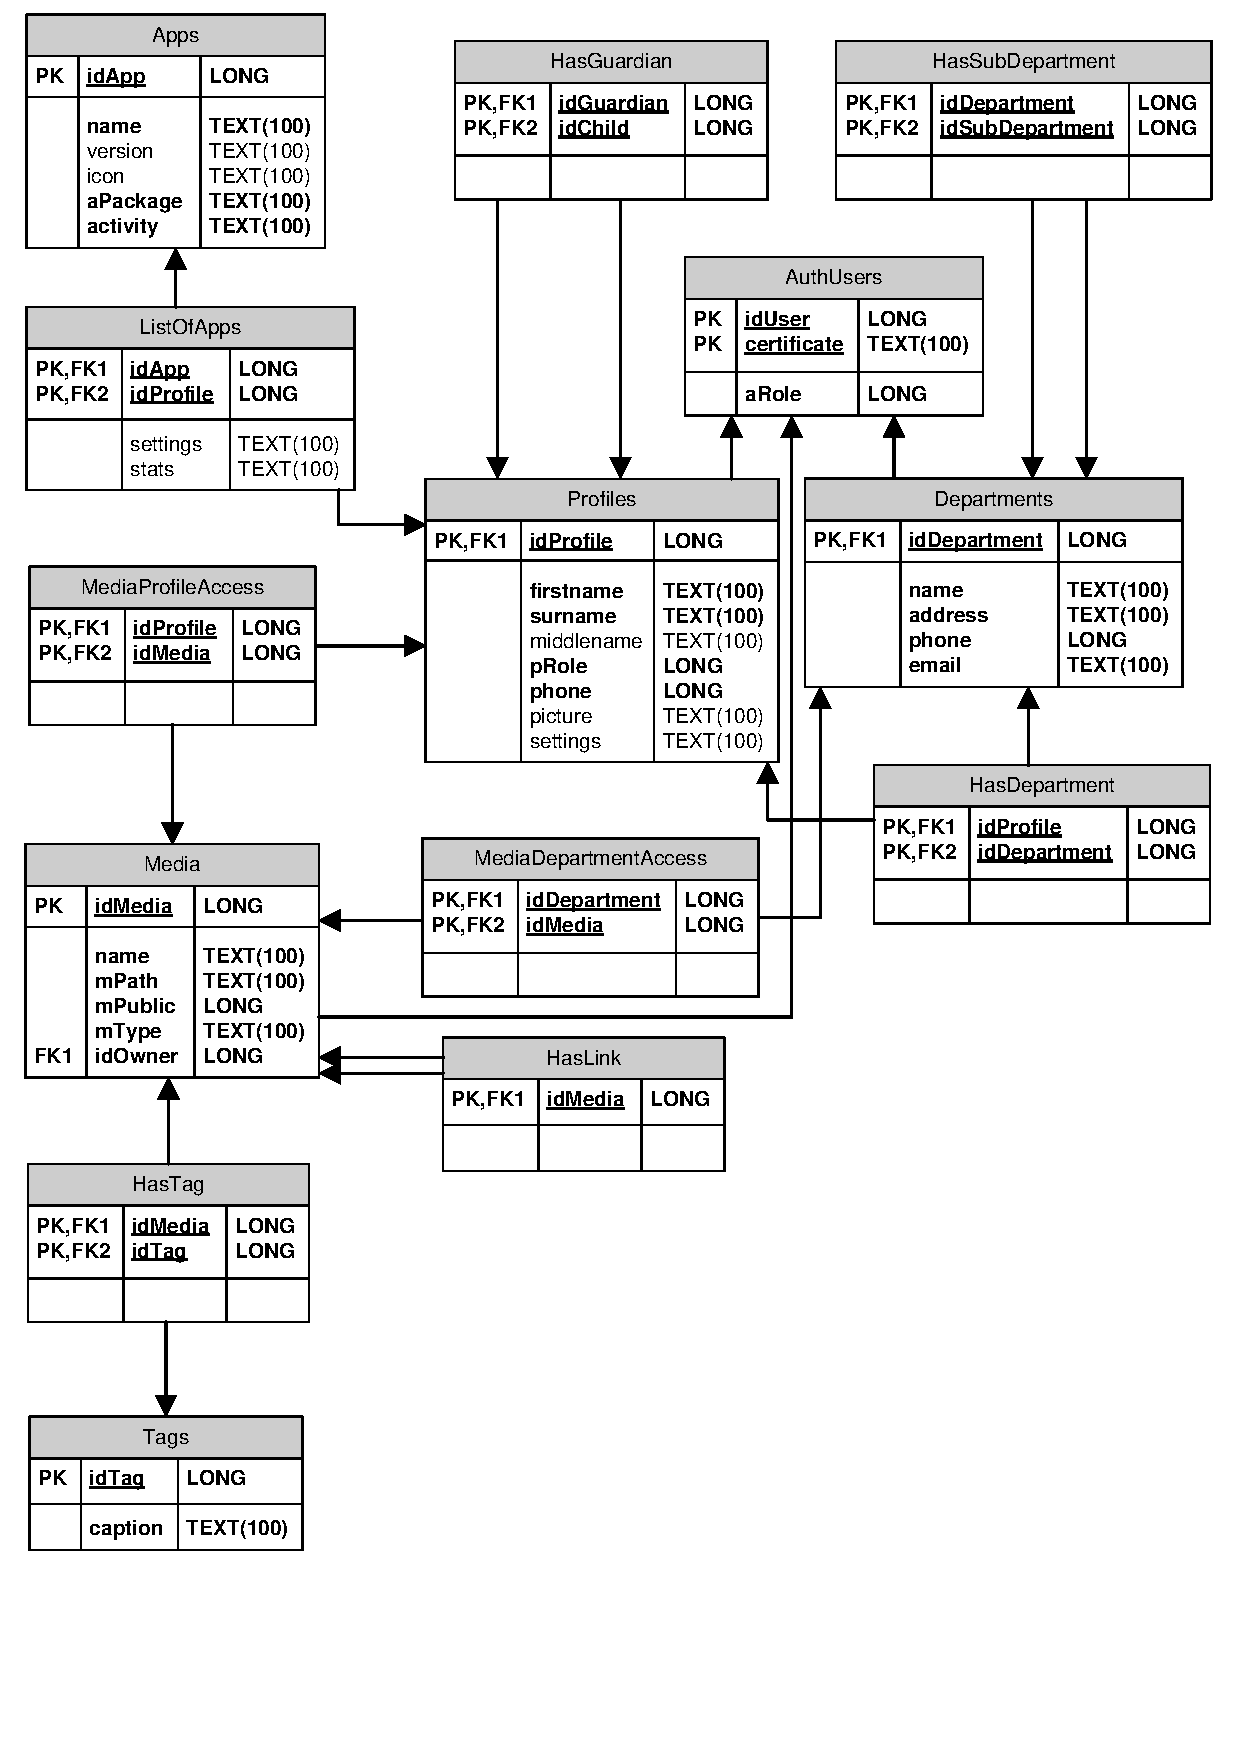
\includegraphics[width=\textwidth]{Images/LocalDatabaseDesign}
	\caption{The database schema for the local database.}
	\label{fig:localDatabaseDesign}
\end{figure}

\section{Implementation}
\label{sec:dbImp}
As said above, we implemented the local database using SQLite. First we made metadata files for each table in the database. The one for the AuthUsers table can be seen in listing \vref{lst:metadata}

\begin{Java}{The AuthUsers MetaData}{lst:metadata}
package dk.aau.cs.giraf.oasis.localdb;

import android.net.Uri;
import android.provider.BaseColumns;

public class AuthUsersMetaData {

	public static final Uri CONTENT_URI = Uri.parse("content://dk.aau.cs.giraf.oasis.localdb.AutismProvider/authusers");

	public static final String CONTENT_TYPE_AUTHUSERS_LIST = "vnd.android.cursor.dir/vnd.dk.authusers";
	public static final String CONTENT_TYPE_AUTHUSER_ONE = "vnd.android.cursor.item/vnd.dk.authusers";

	public class Table implements BaseColumns {
		public static final String TABLE_NAME = "tbl_authusers";

		public static final String COLUMN_ID = "_id";
		public static final String COLUMN_CERTIFICATE = "authusers_certificate";
		public static final String COLUMN_ROLE = "authusers_role";
	}
}
\end{Java}

The uri, CONTENT\_URI and the two strings, CONTENT\_TYPE\_AUTHUSERS\_LIST and CONTENT\_TYPE\_AUTHUSER\_ONE, is not used by the SQLite Database and will be explained later in the content provider section \textcolor{red}{INSERT FIGURE REF}. The inner class Table defines the Strings, which are used as names of the table and the columns.

When the metadata file is created we make a table class file, which defines the SQL statements for creating, updating and deleting the table. The table class file for AuthUsers can be seen in listing \vref{lst:table}.

\begin{Java}{The AuthUsers Table}{lst:table}
package dk.aau.cs.giraf.oasis.localdb;

import android.database.sqlite.SQLiteDatabase;

public class AuthUsersTable {

	private static final String TABLE_CREATE = "CREATE TABLE "
			+ AuthUsersMetaData.Table.TABLE_NAME
			+ "("
			+ AuthUsersMetaData.Table.COLUMN_ID + " INTEGER NOT NULL, "
			+ AuthUsersMetaData.Table.COLUMN_CERTIFICATE + " TEXT NOT NULL, "
			+ AuthUsersMetaData.Table.COLUMN_ROLE + " INTEGER NOT NULL, "
			+ "PRIMARY KEY (" + AuthUsersMetaData.Table.COLUMN_ID + ", " + AuthUsersMetaData.Table.COLUMN_ID + ")"
			+ ");";

	private static final String TABLE_DROP= "DROP TABLE IF EXISTS " + AuthUsersMetaData.Table.TABLE_NAME + ";";

	/**
	 * Executes sql string for creating certificate table
	 * @param db this is an instance of a sqlite database
	 */
	public static void onCreate(SQLiteDatabase db) {
		db.execSQL(TABLE_CREATE);
	}

	/**
	 * executes a sql string which drops the old table and then the method calls oncreate, which create a new certificate table
	 * @param db this is a instance of a sqlite database
	 * @param oldVersion integer referring to the old version number
	 * @param newVersion integer referring to the new version number
	 */
	public static void onUpgrade(SQLiteDatabase db, int oldVersion, int newVersion) {
		db.execSQL(TABLE_DROP);
		onCreate(db);
	}
}
\end{Java}

Now is the Oasis Local Db created, but to be able to access the Oasis Local Db from other applications, it needs to implement a content provider. A content provider allows other applications to fetch data from the application, which implement the content provider. The access to a content provider is done by using a URI, which is defined in the AndroidManifest file. The content provider must implement several methods. These methods are:

\begin{itemize}
	\item onCreate() - called at startup to initialize the content provider.
	\item getType() - called when an application needs to know the type of the data. This is not used in Oasis Local Db.
	\item query() - called when an application wants to query in the Oasis Local Db.
	\item insert() - called when an application wants to insert data into the Oasis Local Db.
	\item update() - called when an application wants to update existing data in the Oasis Local Db.
	\item delete() - called when an application wants to delete existing data in the Oasis Local Db.
\end{itemize}

An example of how we have implemented our content provider, with focus on the authausers table, can be seen in listing \vref{lst:contentprovider}

\begin{Java}{A small part of the content provider}{lst:contentprovider}
package dk.aau.cs.giraf.oasis.localdb;
.
.
.
public class DbProvider extends ContentProvider {

	private DbHelper dbHelper;
	private static final UriMatcher sUriMatcher;
	.
	.
	.
	private static final int AUTHUSERS_TYPE_LIST = 3;
	private static final int AUTHUSERS_TYPE_ONE = 4;
	.
	.
	.
	static {
		sUriMatcher = new UriMatcher(UriMatcher.NO_MATCH);
		.
		.
		.
		sUriMatcher.addURI(DbHelper.AUTHORITY, "authusers", AUTHUSERS_TYPE_LIST);
		sUriMatcher.addURI(DbHelper.AUTHORITY, "authusers/#", AUTHUSERS_TYPE_ONE);
		.
		.
		.
	}
	.
	.
	.
	private static final HashMap<String, String> authusersProjectionMap;
	static {
		authusersProjectionMap = new HashMap<String, String>();
		authusersProjectionMap.put(AuthUsersMetaData.Table.COLUMN_ID, AuthUsersMetaData.Table.COLUMN_ID);
		authusersProjectionMap.put(AuthUsersMetaData.Table.COLUMN_CERTIFICATE, AuthUsersMetaData.Table.COLUMN_CERTIFICATE);
		authusersProjectionMap.put(AuthUsersMetaData.Table.COLUMN_ROLE, AuthUsersMetaData.Table.COLUMN_ROLE);
	}
	.
	.
	.
	@Override
	public boolean onCreate() {
		dbHelper = new DbHelper(getContext());
		return false;
	}

	@Override
	public int delete(Uri uri, String where, String[] whereArgs) {
		SQLiteDatabase db = dbHelper.getWritableDatabase();
		int rowsDeleted = 0;
		String rowId;
		.
		.
		.
		case AUTHUSERS_TYPE_LIST:
			rowsDeleted = db.delete(AuthUsersMetaData.Table.TABLE_NAME, where, whereArgs);
			break;
		case AUTHUSERS_TYPE_ONE:
			rowId = uri.getPathSegments().get(1);
			rowsDeleted = db.delete(AuthUsersMetaData.Table.TABLE_NAME,
					AuthUsersMetaData.Table.COLUMN_ID + " = " + rowId + (!TextUtils.isEmpty(where) ? " AND (" + where + ")" : ""),
					whereArgs);
			break;
		.
		.
		.	
		default:
			throw new IllegalArgumentException("Unknown URI: " + uri);
		}

		getContext().getContentResolver().notifyChange(uri, null);
		return rowsDeleted;
	}

	@Override
	public String getType(Uri uri) {
		switch(sUriMatcher.match(uri)) {
		.
		.
		.
		case AUTHUSERS_TYPE_LIST:
			return AuthUsersMetaData.CONTENT_TYPE_AUTHUSERS_LIST;
		case AUTHUSERS_TYPE_ONE:
			return AuthUsersMetaData.CONTENT_TYPE_AUTHUSER_ONE;
		.
		.
		.
		default:
			throw new IllegalArgumentException("Unknown URI: " + uri);
		}
	}
	@Override
	public Uri insert(Uri uri, ContentValues values) {
		SQLiteDatabase db = dbHelper.getWritableDatabase();
		long rowId;
		Uri _uri;

		switch(sUriMatcher.match(uri)) {
		.
		.
		.
		case AUTHUSERS_TYPE_LIST:
			try {
				rowId = db.insertOrThrow(AuthUsersMetaData.Table.TABLE_NAME, null, values);
				_uri = ContentUris.withAppendedId(AuthUsersMetaData.CONTENT_URI, rowId);
				getContext().getContentResolver().notifyChange(_uri, null);
			} catch (SQLiteConstraintException e) {
				_uri = ContentUris.withAppendedId(AuthUsersMetaData.CONTENT_URI, -1);
			}
			return _uri;
		.
		.
		.
		default:
			throw new IllegalArgumentException("Unknown URI: " + uri);
		}
	}

	@Override
	public Cursor query(Uri uri, String[] projection, String selection, String[] selectionArgs, String sortOrder) {
		SQLiteQueryBuilder builder = new SQLiteQueryBuilder();

		switch(sUriMatcher.match(uri)) {
		.
		.
		.
		case AUTHUSERS_TYPE_LIST:
			builder.setTables(AuthUsersMetaData.Table.TABLE_NAME);
			builder.setProjectionMap(authusersProjectionMap);
			break;
		case AUTHUSERS_TYPE_ONE:
			builder.setTables(AuthUsersMetaData.Table.TABLE_NAME);
			builder.setProjectionMap(authusersProjectionMap);
			builder.appendWhere(AuthUsersMetaData.Table.COLUMN_ID + " = " + uri.getPathSegments().get(1));
			break;
		.
		.
		.
		default:
			throw new IllegalArgumentException("Unknown URI: " + uri);
		}

		SQLiteDatabase db = dbHelper.getReadableDatabase();
		Cursor queryCursor = builder.query(db, projection, selection, selectionArgs, null, null, null);
		queryCursor.setNotificationUri(getContext().getContentResolver(), uri);
		return queryCursor;
	}
	@Override
	public int update(Uri uri, ContentValues values, String where, String[] whereArgs) {
		SQLiteDatabase db = dbHelper.getWritableDatabase();
		int rowsUpdated = 0;
		String rowId;

		switch(sUriMatcher.match(uri)) {
		.
		.
		.
		case AUTHUSERS_TYPE_LIST:
			rowsUpdated = db.update(AuthUsersMetaData.Table.TABLE_NAME, values, where, whereArgs);
			break;
		case AUTHUSERS_TYPE_ONE:
			rowId = uri.getPathSegments().get(1);
			rowsUpdated = db.update(AuthUsersMetaData.Table.TABLE_NAME,
					values,
					AuthUsersMetaData.Table.COLUMN_ID + " = " + rowId + (!TextUtils.isEmpty(where) ? " AND (" + where + ")" : ""),
					whereArgs);
			break;
		.
		.
		.
		default:
			throw new IllegalArgumentException("Unknown URI: " + uri);
		}

		getContext().getContentResolver().notifyChange(uri, null);
		return rowsUpdated;
	}
}
\end{Java}